\documentclass[10pt,a4paper,twocolumn]{article}
\usepackage[T1]{fontenc}
\usepackage[utf8]{inputenc}
\usepackage[a4paper,top=1.9cm,bottom=2.0cm,left=1.75cm,right=1.75cm,columnsep=0.65cm,headheight=14pt]{geometry}
\usepackage{newtxtext,newtxmath}
\usepackage{microtype}
\usepackage{graphicx}
\usepackage{booktabs,array,multirow,tabularx}
\usepackage[table]{xcolor}
\usepackage{caption}
\usepackage{enumitem}
\usepackage{titlesec}
\usepackage{fancyhdr}
\usepackage{placeins}
\usepackage{stfloats}
\usepackage[hidelinks]{hyperref}
\usepackage[nameinlink,noabbrev]{cleveref}

\definecolor{accent}{HTML}{104281}
\hypersetup{colorlinks=true,linkcolor=accent,urlcolor=accent,citecolor=accent}
\graphicspath{{../figures/}}

% every text element is set above 9pt
\newcommand{\tabfont}{\fontsize{9.1}{10.7}\selectfont}
\captionsetup{font={stretch=0.97},labelfont={bf,color=accent},skip=4pt}
\DeclareCaptionFont{capfont}{\fontsize{9.2}{10.8}\selectfont}
\captionsetup{font=capfont}

\titleformat{\section}{\color{accent}\large\bfseries}{\thesection}{0.6em}{}
\titleformat{\subsection}{\color{accent}\normalsize\bfseries}{\thesubsection}{0.5em}{}
\titleformat{\paragraph}[runin]{\normalfont\bfseries}{}{0pt}{}[.]
\titlespacing*{\section}{0pt}{1.1ex plus .4ex}{0.6ex}
\titlespacing*{\subsection}{0pt}{0.9ex plus .3ex}{0.35ex}
\titlespacing*{\paragraph}{0pt}{0.45ex plus .2ex}{0.5em}
\setlist{nosep,leftmargin=1.2em}
\setlength{\parskip}{0.15ex plus 0.1ex}
\setlength{\parindent}{1em}
\setlength{\textfloatsep}{8pt plus 2pt minus 2pt}
\setlength{\floatsep}{7pt plus 2pt minus 2pt}
\setlength{\intextsep}{7pt plus 2pt minus 2pt}
\setlength{\dbltextfloatsep}{8pt plus 2pt minus 2pt}
\setlength{\dblfloatsep}{7pt plus 2pt minus 2pt}
\renewcommand{\topfraction}{0.92}\renewcommand{\dbltopfraction}{0.92}
\renewcommand{\bottomfraction}{0.8}\renewcommand{\textfraction}{0.06}
\renewcommand{\floatpagefraction}{0.8}\renewcommand{\dblfloatpagefraction}{0.8}
\setcounter{topnumber}{4}\setcounter{dbltopnumber}{4}\setcounter{totalnumber}{6}
\emergencystretch=1.5em

\newcommand{\attr}[1]{\texttt{\small #1}}
\newcommand{\code}[1]{\texttt{\small #1}}
\newcommand{\tab}[1]{{\tabfont\setlength{\tabcolsep}{2.2pt}\input{tables/#1}}}
\newcommand{\tabwide}[1]{{\tabfont\setlength{\tabcolsep}{5pt}\input{tables/#1}}}
\newcommand{\tabtight}[1]{{\tabfont\setlength{\tabcolsep}{1.45pt}\input{tables/#1}}}
\newcommand{\eps}{\varepsilon}
\newcommand{\Fm}{F1\textsubscript{mac}}

\pagestyle{fancy}\fancyhf{}
\fancyhead[L]{\small Data Mining 1 -- a.a.\ 2026/2027}
\fancyhead[R]{\small Seller-Level Vehicle Dataset}
\fancyfoot[C]{\thepage}
\renewcommand{\headrulewidth}{0.3pt}

% Fill in the group members (2-3 people) and the delivery date before submitting.
\newcommand{\reportauthors}{Iachim Cristian -- 744069\\}
\newcommand{\reportdate}{December 2026}


\begin{document}
\pagenumbering{roman}
\begin{titlepage}
\onecolumn\centering
\vspace*{3.2cm}
{\large University of Pisa\par}\vspace{0.3cm}
{\large Data Mining 1 -- academic year 2026/2027\par}
\vspace{2.4cm}
{\color{accent}\rule{0.8\linewidth}{1.2pt}\par}\vspace{0.6cm}
{\Huge\bfseries Seller-Level Vehicle Dataset\par}\vspace{0.4cm}
{\LARGE Understanding, segmenting and predicting\\[2pt] the rating of vehicle sellers\par}\vspace{0.6cm}
{\color{accent}\rule{0.8\linewidth}{1.2pt}\par}
\vspace{2.4cm}
{\Large\reportauthors\par}
\vspace{1.2cm}
{\large\reportdate\par}
\vfill
\end{titlepage}
\onecolumn
\tableofcontents
\clearpage
\twocolumn
\pagenumbering{arabic}

\section{Executive summary}\label{sec:intro}
The \emph{Seller-Level Vehicle Dataset} describes 13\,843 vehicle sellers through 24 numerical and 7 categorical attributes aggregated over their listings, plus an identifier and the target \attr{seller\_rating\_class} (\emph{low}, \emph{medium}, \emph{high}). We prepare the data (\cref{sec:m1}), segment the sellers (\cref{sec:m2}), predict the rating and the price (\cref{sec:m3}), mine patterns (\cref{sec:m4}) and connect the results (\cref{sec:concl}). One train/test split, one seed (42) and one clean base are shared by all analyses.

\begin{itemize}
\item \textbf{Structure.} The data are a continuum with two modes, new-car franchises and used-car independents. K-Means with $k=4$ is the finest partition that is reproducible and better than a null model; density-based methods detect anomalies rather than groups.
\item \textbf{Rating.} It is weakly related to the attributes (largest effect size 0.08, cluster ARI $\leq0.025$). Standard grids reach macro-F1 0.41--0.44; a \emph{partial} prior correction and engineered attributes bring KNN to 0.464 (95\% CI 0.443--0.483), level with two ensembles used as a yardstick.
\item \textbf{What drives it.} Seller size, inside every segment. The apparent advantage of independent dealers is a Simpson's paradox.
\item \textbf{Price.} Four attributes explain 91\% of the variance of log price (KNN); mileage alone explains 75\%.
\item \textbf{Patterns.} Rules rediscover the segments, impute the price tertile (75\% vs 35\% accuracy) and predict the rating as well as the baseline models.
\end{itemize}

\section{Data understanding and preparation}\label{sec:m1}

\subsection{Data semantics}\label{sec:sem}
The dataset has 13\,843 rows and 33 columns. Each row is one seller (\attr{sp\_id}); every other column aggregates the listings observed for that seller. \Cref{tab:num} introduces the 24 numerical attributes together with their statistics and \cref{tab:cat} the categorical ones. The target \attr{seller\_rating\_class} is ordinal (\emph{low} $<$ \emph{medium} $<$ \emph{high}); the remaining categorical attributes are nominal. The documentation does not state units: those in \cref{tab:num} are inferred from the value ranges. \attr{sp\_id} is stored as a float but has no fractional part and no repetition, so it was cast to an integer and used only as an index.

Two consequences of the aggregation matter for the whole report. First, each numerical attribute is a \emph{median} over an inventory, so relations that hold car by car need not hold between columns (e.g.\ year $+$ age is not constant). Second, a seller with 5 listings and one with 4\,959 have the same weight, although the medians of the former are far noisier.

\begin{table*}[t]
\centering
\caption{Numerical attributes after cleaning: semantics, statistics, association with the target ($\eps^2$, Kruskal--Wallis effect size) and role in modelling (\emph{log1p}/\emph{raw}: scale used by distance-based and Gaussian methods; \emph{dropped}: eliminated in \cref{sec:corr}). Suffix \attr{\_median} omitted.}\label{tab:num}
\tabtight{m1_numeric}
\end{table*}

\begin{table}[t]
\centering
\caption{Categorical attributes: levels in the raw data, mode, missing values and treatment.}\label{tab:cat}
{\tabfont\setlength{\tabcolsep}{2.5pt}
\begin{tabular}{@{}l r l p{0.35\linewidth}@{}}
\toprule
Attribute & Lev. & Mode (\%) & Missing / treatment\\
\midrule
body\_type & 9 & SUV (64.4) & rare levels merged: 6 groups\\
fuel\_type & 7 & gasoline (98.7) & 1 \emph{unknown} $\to$ NaN; 4 groups\\
transmission & 4 & automatic (93.7) & 6 \emph{unknown} $\to$ NaN\\
wheel\_system & 5 & -- (NaN 76.0) & dropped\\
listing\_color & 11 & white (37.3) & 10.9\% \emph{unknown} kept as level; 8 groups\\
franchise\_status & 2 & franchise (50.6) & none\\
new\_used\_profile & 3 & used only (53.3) & none; function of \attr{pct\_is\_new}\\
rating\_class & 3 & medium (54.7) & target\\
\bottomrule
\end{tabular}}
\end{table}

\subsection{Distributions and statistics}
\paragraph{Target} The classes are imbalanced (\cref{fig:target}, left): 54.7\% \emph{medium}, 26.6\% \emph{high}, 18.6\% \emph{low}. A majority predictor already scores 0.547 accuracy, so \cref{sec:m3} uses stratified splits and selects models by macro-F1. The dealer type shifts the mix (\cref{fig:target}, right): independents are rated \emph{high} more often than franchises (33\% vs 21\%) and \emph{low} less often (16\% vs 21\%). The association is significant ($\chi^2=270$, $p<10^{-58}$) but weak (Cram\'er's $V=0.14$).

\begin{figure*}[t]
\centering
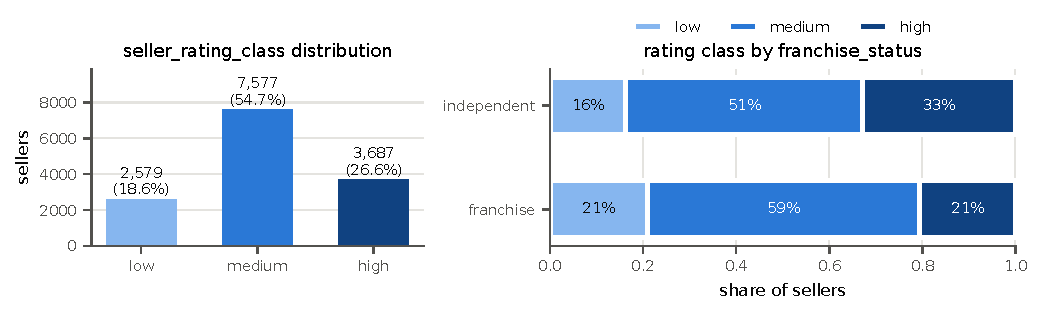
\includegraphics[width=0.92\textwidth]{m1_target_balance}
\caption{Class balance of the target (left) and rating mix by dealer type (right).}\label{fig:target}
\end{figure*}

\paragraph{Numerical attributes} Three shapes dominate \cref{tab:num,fig:log}. Volumes, prices and times are strongly right-skewed (\attr{daysonmarket} 8.8, \attr{city\_fuel\_economy} 8.1, \attr{n\_listings} 5.2). Inventory-mix shares are zero-inflated: 91\% of the sellers have no salvage vehicle, 85\% no theft title. \attr{pct\_is\_new} and \attr{mileage} are bimodal: 53\% of the sellers list no new car, while the rest form a new-car mode at almost zero mileage. This used/new duality is the main structure of the data and reappears in every module.

\begin{figure*}[t]
\centering
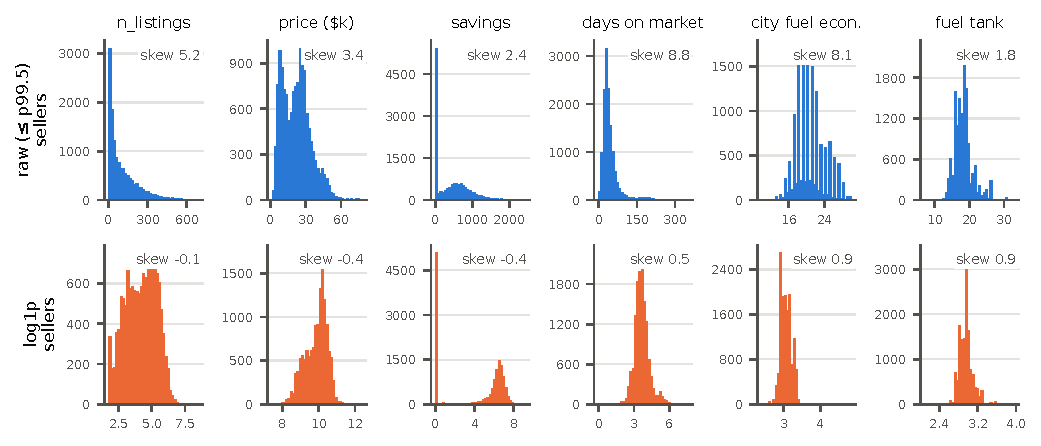
\includegraphics[width=0.97\textwidth]{m1_log_transform}
\caption{Log-transformed modelling attributes, raw scale clipped at $p_{99.5}$ (top) and \code{log1p} scale (bottom). \attr{savings\_amount} keeps its spike at zero: 37\% of the sellers advertise no savings.}\label{fig:log}
\end{figure*}

\begin{figure*}[t]
\centering
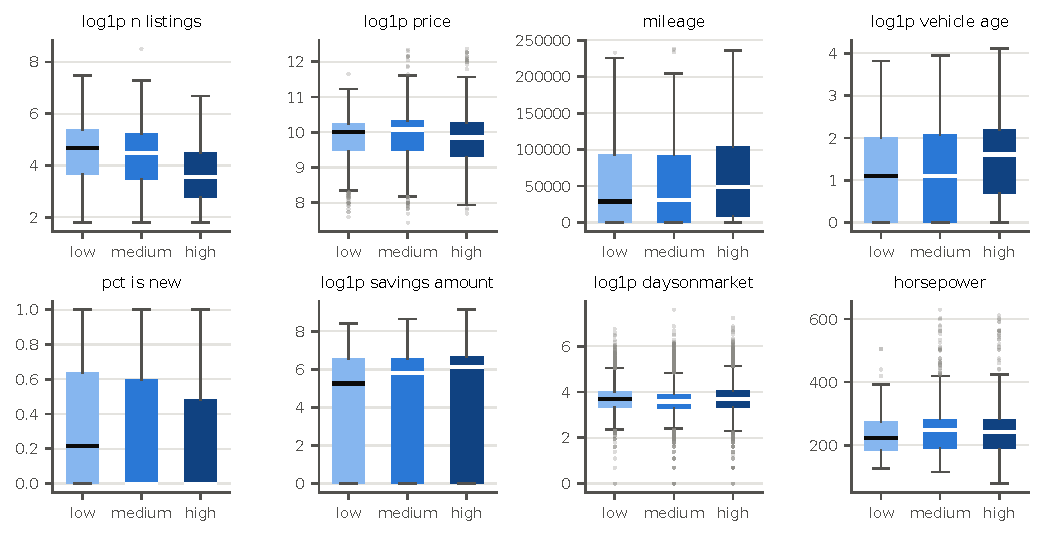
\includegraphics[width=0.97\textwidth]{m1_box_by_target}
\caption{Key attributes by rating class. Only seller size (\attr{n\_listings}) separates the classes visibly, and mainly \emph{high} from the other two.}\label{fig:box}
\end{figure*}

\paragraph{Attributes vs target} We used Kruskal--Wallis tests because of the skew. With 13\,843 sellers every attribute except \attr{front\_legroom} ($p=0.07$) is significant, so we read effect sizes instead of $p$-values ($\eps^2$ in \cref{tab:num}). Seller size is the only attribute with a moderate effect (\attr{n\_listings} $\eps^2=0.082$, \attr{n\_listing\_days} 0.073); all others are at most 0.017. Median size drops from 107 (\emph{low}) and 88 (\emph{medium}) to 34 listings for \emph{high} (\cref{fig:box}). High-rated sellers are typically small, used-car, independent dealers; \emph{low} and \emph{medium} overlap almost completely. This sets modest expectations for \cref{sec:m3}.

\paragraph{Categorical attributes} Most levels are very concentrated (\cref{fig:cat}): \attr{fuel\_type} and \attr{transmission} are almost constant, body type is dominated by SUVs, and colour by white and black. Only 31 sellers (0.2\%) sell new cars only. \attr{franchise\_status} shows just two of the four documented levels (\emph{mixed} and \emph{unknown} never occur).

\begin{figure*}[t]
\centering
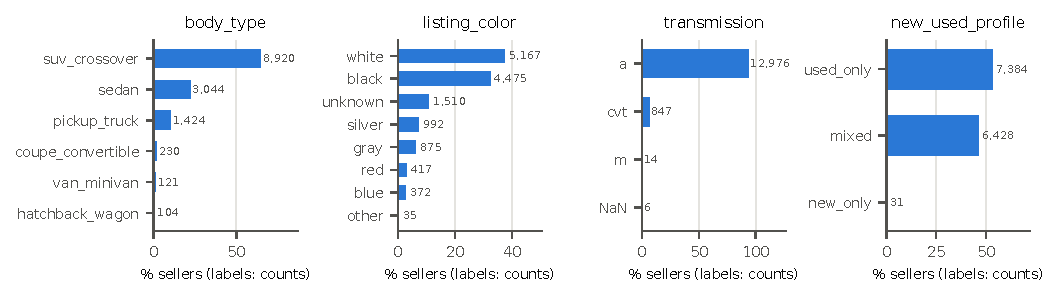
\includegraphics[width=0.97\textwidth]{m1_categorical}
\caption{Categorical attributes after the grouping of rare levels (labels: number of sellers).}\label{fig:cat}
\end{figure*}

\subsection{Data quality}\label{sec:quality}
\paragraph{Duplicates} There are no duplicate rows, no duplicate \attr{sp\_id}, and no two sellers with identical attributes.

\paragraph{Missing values} We looked for explicit \code{NaN} and for implicit codes (\emph{unknown}, empty strings, impossible zeros). Zeros are legitimate for savings, mileage, age, days on market, span and shares. Three attributes have relevant missingness (\cref{fig:miss}); all others are below 0.3\%. We tested whether missingness depends on the target or dealer type, because that decides between dropping and imputing:
\begin{itemize}
\item \attr{wheel\_system} (76.0\%): independent of the target ($\chi^2$ $p=0.32$) and of dealer type ($p=0.17$). Imputing it would invent three quarters of the column, so it was \textbf{dropped}.
\item \attr{engine\_displacement} (24.5\%): also independent of target ($p=0.21$) and dealer ($p=0.61$); \textbf{excluded} from modelling because of its missing rate and redundancy (\cref{sec:corr}).
\item \attr{listing\_color} = \emph{unknown} (10.9\%): 15.9\% for franchises but 5.8\% for independents ($p<10^{-80}$). The absence is informative, so it was \textbf{kept as a level}.
\end{itemize}
The 27 missing \attr{pct\_isCab}, \attr{pct\_salvage} and \attr{pct\_theft\_title} occur in the same rows, all (almost) new-only sellers. This missingness is structural (a new car cannot be an ex-taxi or a salvage), so they were set to 0 by rule.

The remaining \code{NaN}s are \emph{not} imputed here. Imputing on the whole dataset would leak test information into \cref{sec:m3}: medians and modes are fitted on all data only for the unsupervised analyses, and inside the training folds for supervised ones.

\begin{figure}[t]
\centering
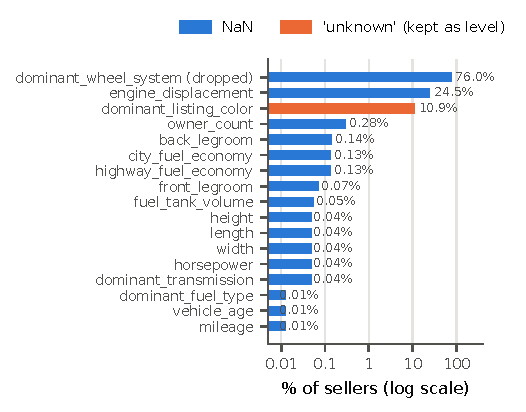
\includegraphics[width=0.92\linewidth]{m1_missing}
\caption{Missing values per attribute (log scale).}\label{fig:miss}
\end{figure}

\paragraph{Consistency checks} We evaluated 14 rules (\cref{tab:checks}). Only two reveal errors, and both were set to \code{NaN}; the others have a domain explanation that we checked on the records. For example, the 338 majority-new sellers with mileage above 5\,000 have a median vehicle age of 0: \attr{is\_new} marks recent model years, not zero-kilometre cars.

\begin{table}[t]
\centering
\caption{Consistency rules. No violation was found for negative values, shares outside $[0,1]$, \attr{new\_used\_profile} vs \attr{pct\_is\_new}, listing days vs listings/span, and savings $>$ price.}\label{tab:checks}
{\tabfont\setlength{\tabcolsep}{3pt}
\begin{tabular}{@{}p{0.43\linewidth}r p{0.41\linewidth}@{}}
\toprule
Rule violated & $n$ & Decision\\
\midrule
front legroom $>46$ in & 2 & error $\to$ NaN (54 and 67 in on SUVs)\\
non-electric economy $>60$ MPG & 2 & error $\to$ NaN (petrol, 210--388 hp)\\
\midrule
electric economy $>60$ & 8 & kept: MPGe unit\\
highway $<$ city economy & 18 & kept: hybrids, mixed stock\\
rear legroom $=0$ & 3 & kept: two-seat pickups, vans\\
model year $<1995$ & 38 & kept: classic-car dealers\\
year $+$ age $\notin[2018,2022]$ & 42 & kept: medians not additive\\
share new $>0.5$, mileage $>5$k & 338 & kept: recent model years\\
days on market $>$ span & 120 & kept: listed before window\\
\bottomrule
\end{tabular}}
\end{table}

\paragraph{Outliers} The $1.5\,$IQR rule on the modelling scale flags between 0\% and 6.7\% of the values of the continuous attributes (\attr{length} 6.7\%, \attr{daysonmarket} 6.1\%, \attr{fuel\_tank} 4.8\%). It is meaningless for zero-inflated shares, where $\mathrm{IQR}=0$ flags every non-zero value (15\% for \attr{pct\_theft\_title}). The extremes we inspected are real sellers: supercar dealers (up to \$236k), classic-car dealers (median \$34.9k vs \$22.3k), a 4\,959-listing dealer, heavy-duty trucks. We therefore \textbf{kept} all of them and limited their influence through log scales. Multivariate anomalies are analysed as DBSCAN noise (\cref{sec:dbscan}), and the effect of keeping them is measured in \cref{sec:m2core,sec:ablation}.

\subsection{Variable transformations}\label{sec:trans}
We applied \code{log1p} when the raw skewness exceeds 1 \emph{and} the log at least halves it; otherwise the transform only costs interpretability. This selects nine attributes (\attr{n\_listings}, \attr{price}, \attr{savings}, \attr{daysonmarket}, both fuel economies, \attr{fuel\_tank}, \attr{engine\_displacement}, \attr{vehicle\_age}) and rejects e.g.\ \attr{listing\_span} (2.15 $\to$ $-1.22$, over-corrected) and \attr{mileage} (bimodal, $0.68\to-0.91$). Rare categorical levels ($<1\%$) were merged by meaning (e.g.\ coupe $+$ convertible), because they produce unstable splits and itemsets.

Each task uses its own view of the same clean base: log $+$ standardized for distances and Gaussians (K-Means, DBSCAN, KNN, GaussianNB), raw for trees (invariant to monotone transforms), binned for CategoricalNB and pattern mining. Whether these choices matter is tested by ablation in \cref{sec:m2attr,sec:ablation}.

\subsection{Pairwise correlations and elimination}\label{sec:corr}
Spearman's $\rho_s$ is the main criterion, since relations are monotone but not linear (price--mileage: $r=-0.68$, $\rho_s=-0.82$). \Cref{fig:heat} shows two blocks: \emph{newness} (mileage, year, age, owners, share of new, price) and \emph{vehicle size and power} (horsepower, displacement, tank, dimensions, and inversely fuel economy). \Cref{tab:corr} lists the strongest pairs.

\begin{figure*}[t]
\centering
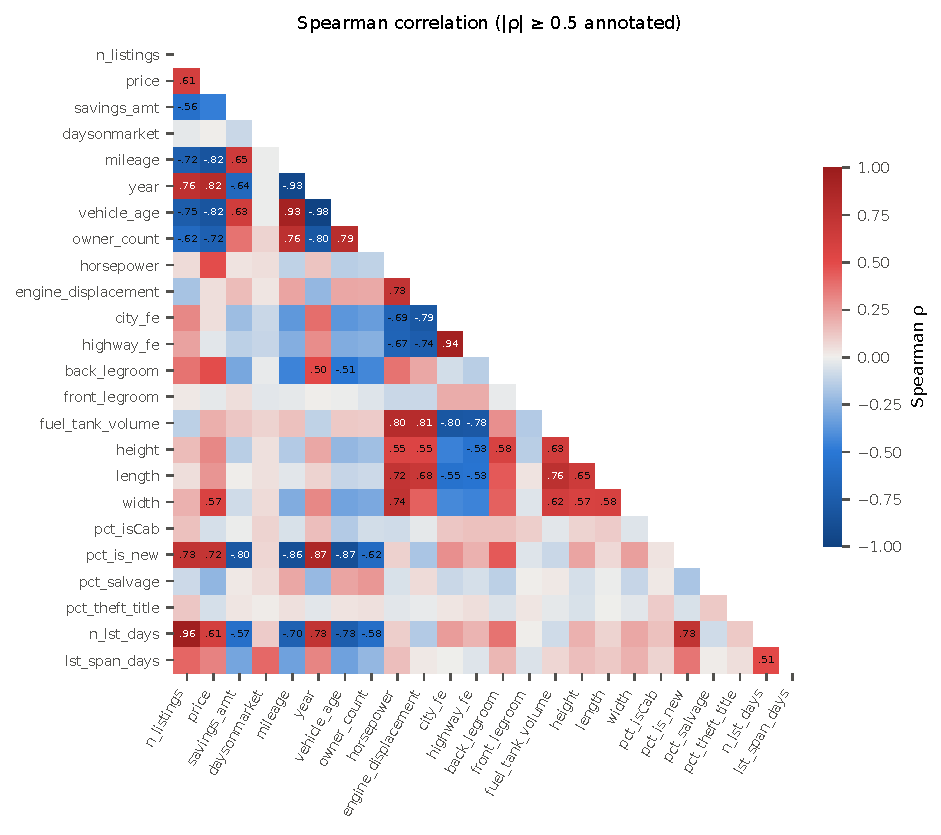
\includegraphics[width=0.80\textwidth]{m1_spearman_heatmap}
\caption{Spearman correlations of the 24 numerical attributes ($|\rho_s|\geq0.5$ annotated).}\label{fig:heat}
\end{figure*}

\begin{table}[t]
\centering
\caption{Pairs with $\max(|r|,|\rho_s|)\geq0.8$.}\label{tab:corr}
\tab{m1_corr}
\end{table}

A pair with $|\rho_s|\geq0.90$ is redundant and loses one member: \attr{year} and \attr{vehicle\_age} in favour of \attr{mileage} (continuous, least skewed wear measure), \attr{n\_listing\_days} in favour of \attr{n\_listings}, and highway in favour of city fuel economy. We also drop \attr{engine\_displacement} (missing rate; $\rho_s=0.81$ with \attr{fuel\_tank}) and \attr{new\_used\_profile} (a discretization of \attr{pct\_is\_new}). \attr{mileage} and \attr{pct\_is\_new} ($-0.86$) are both kept: they are under the threshold and describe wear and inventory mix. The criterion never looks at the target, so it cannot leak. The modelling set has \textbf{19 numerical and 5 categorical attributes}. \attr{franchise\_status} and \attr{new\_used\_profile} are almost equivalent ($V=0.90$), which is one more reason to keep only the former; the 680 sellers that break the pattern (610 used-only franchises, 70 mixed independents) remain visible through \attr{pct\_is\_new}.

\section{Clustering}\label{sec:m2}
\attr{sp\_id} and \attr{seller\_rating\_class} never enter the clustering; the target is only used afterwards as an external label.

\subsection{Attributes and preprocessing}\label{sec:m2attr}
We cluster seven attributes that describe \emph{how a seller does business}: size (\attr{n\_listings}), market segment (\attr{price}), discounting (\attr{savings\_amount}), turnover (\attr{daysonmarket}), wear (\attr{mileage}), composition (\attr{pct\_is\_new}) and activity period (\attr{listing\_span}). The first four are log-transformed, all are standardized, and the single missing mileage is median-imputed.

The other attributes are left out on purpose and used for profiling. Vehicle specifications describe the cars and not the business, and their mutual correlation would let them dominate the distance as a block. Zero-inflated shares become artificial outliers once standardized. Mixing one-hot categoricals with continuous attributes would require an arbitrary weight. \Cref{tab:sens} supports the choice: with all 19 attributes the silhouette never exceeds 0.22 (distance concentration), and three extra specifications already lower it at every $k$. The raw scale sometimes scores higher, but by isolating extremes (at $k=3$ a group of 739 sellers), so the log view is kept.

\begin{table}[t]
\centering
\caption{K-Means silhouette by attribute set and scale (min$_4$: smallest cluster at $k=4$). The row used is the first one.}\label{tab:sens}
\tab{m2_sens}
\end{table}

\subsection{Centroid-based clustering}\label{sec:kmeans}
\paragraph{Choice of $k$} We ran K-Means for $k=2,\dots,12$ (\code{n\_init}$=10$, k-means++) and Bisecting K-Means (splitting the largest cluster), recording SSE, silhouette and Davies--Bouldin (\cref{fig:ksweep}). $k=2$ has the best silhouette (0.42) but only separates new-car from used-car sellers, which \attr{new\_used\_profile} already states (ARI 0.83). Among $k>2$, $k=4$ is the best on \emph{both} silhouette (0.343) and Davies--Bouldin (1.17); the SSE flattens after it, the smallest cluster still holds 9\% of the sellers, and from $k=6$ the silhouette falls below 0.25. Bisecting K-Means equals K-Means at $k=2$ and is worse afterwards (silhouette 0.26 at $k=4$): its greedy splits cannot be revised.

\begin{figure*}[t]
\centering
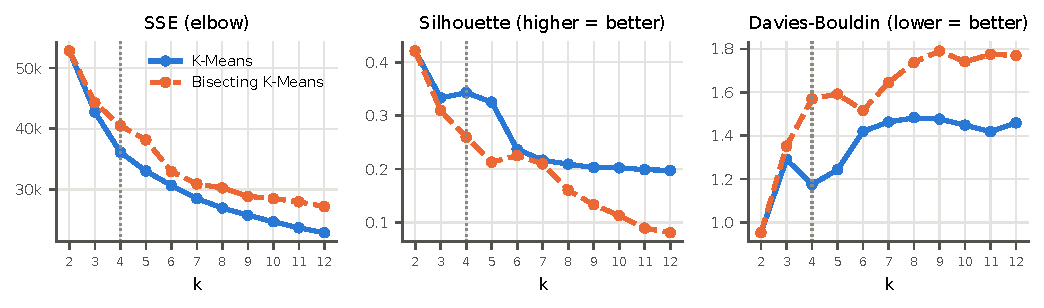
\includegraphics[width=0.95\textwidth]{m2_kmeans_sweep}
\caption{K-Means and Bisecting K-Means for $k=2,\dots,12$. Dotted line: chosen $k=4$.}\label{fig:ksweep}
\end{figure*}

\paragraph{Null model and stability} A silhouette of 0.34 is hard to judge alone, so we compared it with a null model: 20 datasets with each column permuted independently (same marginals, no dependence) and clustered in the same way (\cref{fig:validity}). The null silhouette is $0.14$--$0.16$ at every $k$ and never exceeds 0.165, so the structure is real for all $k$; but its margin falls from 0.20 at $k=4$ to 0.07 at $k=8$, and SSE relative to the null stops improving after $k=4$ (0.63, 0.56, \textbf{0.51}, 0.50, 0.49). As a second check we clustered pairs of 80\% subsamples and compared the labels of the common sellers (20 pairs per $k$): ARI is $\geq 0.99$ for $k\leq4$, then becomes unstable ($0.97\pm0.07$ at $k=5$, $0.90\pm0.15$ at $k=6$). Both checks point to $k=4$ as the finest reproducible partition.

\begin{figure*}[t]
\centering
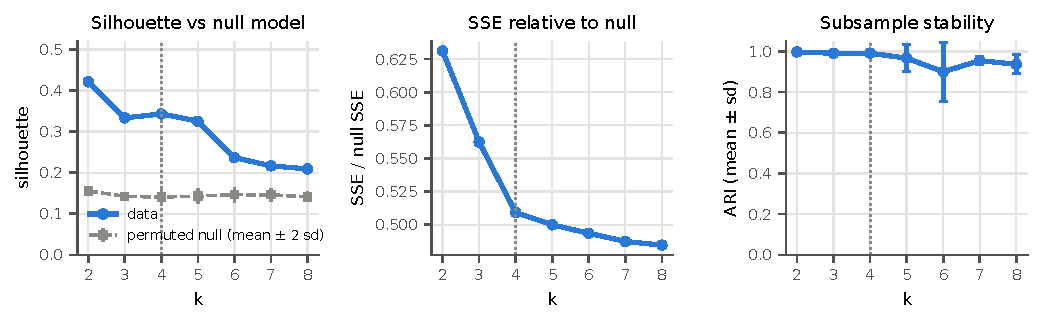
\includegraphics[width=0.95\textwidth]{m5_cluster_validity}
\caption{Cluster validity of K-Means: silhouette against 20 column-permuted null datasets, SSE relative to the null, and ARI between clusterings of random 80\% subsamples.}\label{fig:validity}
\end{figure*}

\paragraph{X-Means} We also implemented X-Means, which splits a cluster when the BIC of two spherical Gaussians beats one. It never stops on its own: $k$ grows 2, 4, 8, 15, 27, 41, 57 and reaches our cap of 64 with 20 splits still accepted. With almost 14\,000 sellers the BIC penalty is negligible against any departure from a spherical Gaussian. This is an informative negative result: the data are a continuum that can be refined indefinitely, so an automatic criterion does not replace the analysis above.

\paragraph{Profiles} \Cref{tab:prof,fig:kprof} describe the four segments, numbered by decreasing price:
\begin{itemize}
\item \textbf{C0 -- franchise new-car dealers} (37\%): large, almost zero mileage, 65\% new cars, high price, no advertised savings.
\item \textbf{C1 -- mid-market used dealers} (26\%): late-model cars ($\approx$33k miles), regular discounting; half franchise, half independent.
\item \textbf{C2 -- slow-turnover dealers} (9\%): old stock listed for 92 days against 32--39 elsewhere, over a long activity span.
\item \textbf{C3 -- small budget independents} (28\%): few listings, $\approx$113k miles, the lowest prices.
\end{itemize}
\Cref{fig:kscatter} shows that the segments occupy contiguous regions with blurred borders, not separate clouds. The rating is spread over all of them (ARI 0.014), yet the share of \emph{high} grows from 20\% in C0 to 34--36\% in C2 and C3.

\begin{table}[t]
\centering
\caption{K-Means $k=4$: cluster medians in original units (top), composition and rating mix (bottom).}\label{tab:prof}
\tab{m2_profiles}
\end{table}

\begin{figure*}[t]
\centering
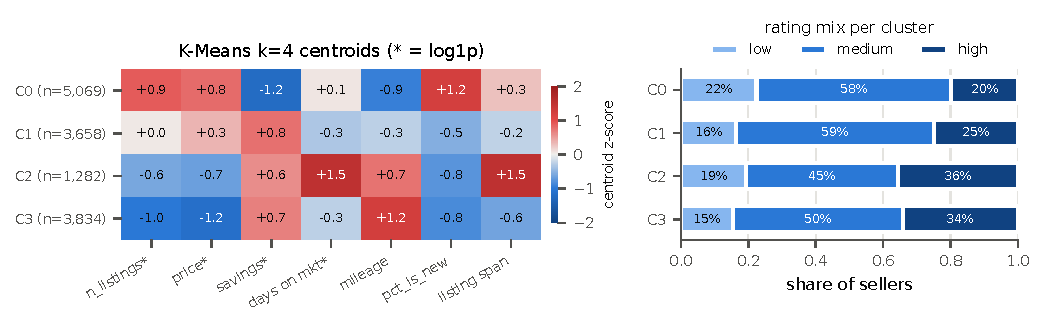
\includegraphics[width=0.95\textwidth]{m2_kmeans4_profile}
\caption{K-Means $k=4$: standardized centroids (left; * = log scale) and rating mix per segment (right).}\label{fig:kprof}
\end{figure*}

\begin{figure*}[t]
\centering
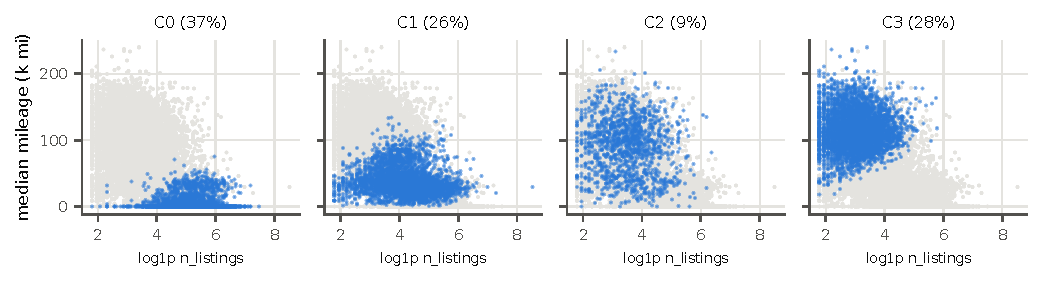
\includegraphics[width=0.93\textwidth]{m2_kmeans4_scatter}
\caption{Each K-Means segment highlighted over all sellers, in two original dimensions (size and mileage).}\label{fig:kscatter}
\end{figure*}

\subsection{Density-based clustering}\label{sec:dbscan}
\paragraph{Parameters} We kept the seven attributes: more dimensions would concentrate distances and make one global $\eps$ even harder to set. The heuristic MinPts $\approx 2d=14$ suggests the range $\{5,10,15,20,30\}$. The $k$-distance graphs (\cref{fig:kdist}) rise smoothly, without a sharp knee, between 0.35 and 1.0, which is our range for $\eps$. \Cref{tab:dbscan} reports all 45 configurations. Values at the classical knee ($\eps\geq0.7$) merge everything into one cluster; small values produce many micro-clusters and up to 87\% noise.

\begin{figure}[t]
\centering
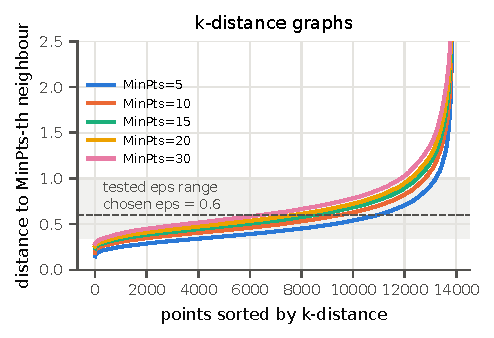
\includegraphics[width=0.94\linewidth]{m2_kdistance}
\caption{$k$-distance graphs on the seven standardized attributes, with the tested and the chosen $\eps$.}\label{fig:kdist}
\end{figure}

\begin{table*}[t]
\centering
\caption{DBSCAN, all tested configurations. Each cell: number of clusters (of which with $\geq1\%$ of the sellers); noise; silhouette on non-noise points (--: one cluster).}\label{tab:dbscan}
\tabwide{m2_dbscan}
\end{table*}

The silhouette alone would reward discarding points (0.69 with 87\% noise), so we selected, among the configurations with at least two clusters of $\geq1\%$ of the sellers, the one with the \textbf{lowest noise}: $\eps=0.6$, MinPts $=15$, with two clusters, 22\% noise and silhouette 0.49 on the retained points.

\paragraph{Result} The two dense cores are used-car dealers (D0, 6\,542, mostly C1 and C3) and franchise new-car dealers (D1, 4\,256, all from C0): the K-Means $k=2$ split. D0 has a median of 37 listings, 79k miles and \$15.2k, with 24\% franchises; D1 has 193 listings, 11 miles and \$29.8k, with 66\% new cars and only franchises. The share of \emph{high} is 29\% in D0, 19\% in D1 and 33\% in the noise. \Cref{tab:noise} characterizes the 3\,045 noise sellers: they are not corrupted records. Slow turnover dominates (a median above 120 days on market is 76 times more frequent than in the cores; 77\% of C2 is noise), followed by extreme prices and tiny inventories (ratio 3--4). Large sellers are not over-represented.

\begin{table}[t]
\centering
\caption{Traits of DBSCAN noise vs core sellers.}\label{tab:noise}
\tab{m2_noise}
\end{table}

\paragraph{OPTICS} The reachability plot (\cref{fig:optics}, MinPts $=15$) shows two broad valleys, the two cores, separated by a short rise, and then a steady climb through the noise. Cutting it at 0.6 reproduces DBSCAN (ARI 0.999), while the $\xi$ method ($\xi=0.05$), which needs steep walls, returns a single cluster. Density varies continuously, so a density-based method has no natural threshold here.

\begin{figure}[t]
\centering
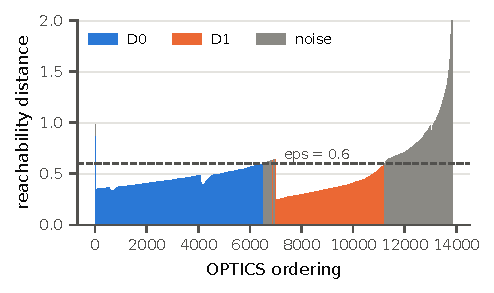
\includegraphics[width=0.94\linewidth]{m2_optics_reachability}
\caption{OPTICS reachability plot, coloured by DBSCAN label.}\label{fig:optics}
\end{figure}

\subsection{Sensitivity of K-Means to outliers}\label{sec:m2core}
We refitted K-Means ($k=4$) on the DBSCAN core points and assigned all sellers to the new centroids: ARI 0.79 with the original partition. C0 and C1 survive unchanged; C2 disappears, because its members are mostly noise, and the freed centroid splits C3. C2 is therefore a real but \emph{sparse} segment, defined by its tail behaviour. We keep it for its business meaning and report this caveat.

\subsection{Hierarchical clustering}
We clustered all 13\,843 sellers with seven linkage/distance pairs: Single, Complete, Average and Ward with Euclidean distance (Ward minimizes the within-cluster variance increase and is defined only for it), Complete and Average with Manhattan (less sensitive to one large difference), and Average with cosine (profile shape, ignoring magnitude). \Cref{fig:dendro} shows six dendrograms, \cref{tab:hier} the cophenetic correlation $r_c$ and the silhouette of the cuts (computed with the same distance).

\begin{figure*}[t]
\centering
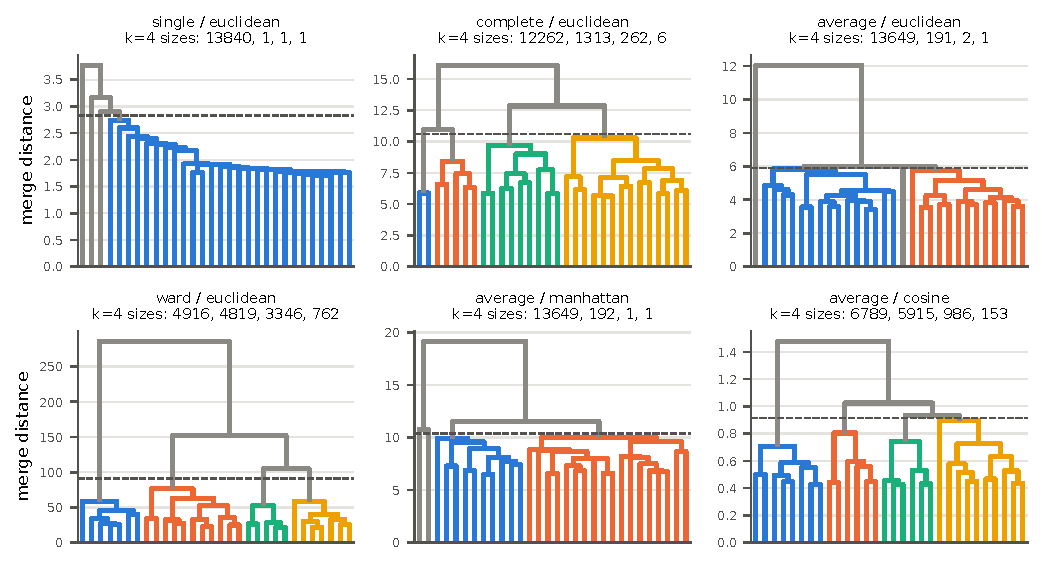
\includegraphics[width=0.95\textwidth]{m2_dendrograms}
\caption{Dendrograms (last 30 merges). Dashed line: height that gives four clusters, whose sizes are in the titles.}\label{fig:dendro}
\end{figure*}

\begin{table}[t]
\centering
\caption{Hierarchical clustering: cophenetic correlation, silhouette of the cuts $k=2,\dots,6$, and extreme cluster sizes at $k=4$.}\label{tab:hier}
\tabtight{m2_hier}
\end{table}

\textbf{Single} linkage chains: its $k=4$ cut is one giant cluster plus three singletons, and its silhouette (0.53) is an artefact of isolating outliers. \textbf{Average} (Euclidean and Manhattan) has the same defect in milder form. \textbf{Complete} is driven by maximum distances: 89\% of the sellers fall in one cluster. \textbf{Cosine/Average} has the best $r_c$ (0.86) and a balanced $k=2$ cut, but it ignores how far a seller is from the mean profile and adds a 153-seller fringe. \textbf{Ward} gives compact, balanced clusters. Its last merge heights (63, 76, 105, 152, 286) have the largest gap at the new/used split; the gap above four clusters ($76\to105$) is still twice the next one ($63\to76$), so we cut at $k=4$. The result resembles K-Means (ARI 0.76): W0 (35\%, 187 listings, \$30.1k, 100\% franchises) is C0; W1 (24\%, 31k miles, \$24.0k) is C1; W3 (36\%, 21 listings, 109k miles, \$10.3k) is C3 enlarged with parts of C1 and C2; W2 keeps only 762 sellers (6\%), identified by a long activity span (median 949 days) more than by slow turnover (63 days on market). The rating mix moves as in K-Means: \emph{high} is 20\% in W0 and 34\% in W3.

\subsection{Comparison and best algorithm}
\begin{table*}[t]
\centering
\caption{Final comparison. For DBSCAN, internal and external indices refer to non-noise points only, hence optimistic; SSE is comparable only at equal $k$. ARI$_\mathrm{KM4}$: agreement with the chosen K-Means partition.}\label{tab:cmp}
\tabtight{m2_comparison}
\end{table*}

\paragraph{Geometry} All evidence (soft elbow, silhouettes $\leq0.42$, no steep valley in OPTICS, unbounded X-Means, 22\% noise needed to separate two modes) describes a \emph{continuum with two broad density modes}, new/franchise and used/independent, plus a sparse slow-turnover tail.

\paragraph{Best algorithm} Given this geometry, a partition of the continuum is more useful than a search for separated shapes. \textbf{K-Means with $k=4$ is our choice}: in \cref{tab:cmp} it has the best internal indices among non-degenerate $k=4$ partitions, it covers every seller, it is reproducible (ARI $\geq0.998$ across 10 seeds, 0.99 across subsamples), and its segments are easy to read. Ward agrees and adds the nesting (new vs used first), at a much higher memory cost. Bisecting K-Means is dominated. DBSCAN and OPTICS are a poor segmentation tool here but a good anomaly detector. No partition aligns with the rating (ARI $\leq0.025$): business type only \emph{shifts} the rating mix, which anticipates the low ceiling of \cref{sec:m3}. The segments are reused to analyse errors and size effects (\cref{sec:errors}) and are turned into rules in \cref{sec:segrules}.

\section{Classification and regression}\label{sec:m3}

\subsection{Experimental design}
The target is \attr{seller\_rating\_class}, predicted from the 19 numerical and 5 categorical attributes of \cref{sec:corr}. One stratified 80/20 split (11\,074 / 2\,769 sellers, seed 42) is shared by every classifier, by the regressions and by the rules of \cref{sec:exploit}. All tuning uses stratified 5-fold CV on the training set, with imputation, log, scaling, encoding and binning refitted \emph{inside} each fold. We select by \textbf{macro-F1}, which weighs the three classes equally; the majority class scores 0.236 (accuracy 0.547), stratified random guessing 0.334. The way to handle imbalance is itself a hyperparameter of each model.

\subsection{Baseline grids}\label{sec:grids}
\Cref{tab:grids} lists all tested values (658 configurations), with the best CV macro-F1 each value reaches.

\begin{table*}[t]
\centering
\caption{Baseline grids: tested values, each followed by the best CV macro-F1 over the rest of the grid (bold: chosen).}\label{tab:grids}
{\tabfont\setlength{\tabcolsep}{4pt}
\begin{tabular}{@{}l l p{0.655\textwidth}@{}}
\toprule
Model (configs) & Parameter & Values (best CV macro-F1)\\
\midrule
Decision Tree (432) & criterion & \textbf{gini} .419, entropy .406\\
 & max depth & 2 .392, 3 .395, 4 .367, \textbf{5} .419, 6 .411, 8 .409, 10 .412, 12 .411, none .411\\
 & min samples leaf; split & leaf: 1 .417, 5 .417, 20 .419, \textbf{50} .419; split: \textbf{2}, 20, 100 all .419\\
 & class weight & none .407, \textbf{balanced} .419\\
\midrule
KNN (128) & $k$ & 1 .390, 3 .388, 5 .392, 7 .387, 9 .392, 11 .402, 15 .409, 21 .415, 31 .416, 41 .424, 51 .424, 75 .429, 101 .434, \textbf{151} .434, 201 .433, 301 .429\\
 & Minkowski $p$; weights & $p$: \textbf{1} .434, 2 .434; weights: uniform .432, \textbf{distance} .434\\
 & decision rule & plain vote .390, \textbf{prior-corrected} .434\\
\midrule
GaussianNB (26) & var.\ smoothing; priors & $10^{-12}$--$10^{-3}$ .403, $10^{-2}$ .403, $\mathbf{10^{-1}}$ .404, 1 .400; priors: empirical .391, \textbf{uniform} .404\\
CategoricalNB (72) & bins; $\alpha$; priors & bins: \textbf{3} .416, 4 .413, 5 .412, 6 .414, 8 .412, 10 .412; $\alpha$: \textbf{0.01}--5 all .415--.416; priors: \textbf{empirical} .416, uniform .404\\
\bottomrule
\end{tabular}}
\end{table*}

\paragraph{Decision Tree} Inputs are not scaled (splits are invariant). Depth and class weighting matter; criterion and minimum split size hardly do. \Cref{tab:prune,fig:overfit} show overfitting control: the unpruned tree (3\,350 leaves) memorizes the training set (F1 1.00) and reaches 0.387 in CV; pre-pruning at depth 5 (31 leaves) gives 0.419 with a small gap. Cost-complexity pruning (40 $\alpha$ values along the pruning path) peaks at $\alpha=4.5\cdot10^{-4}$, with 93 leaves, and stays below (0.401). The depth curve has a dip at 4 and a flat tail, so it reads ``shallow is enough'' and not ``exactly 5''.

\begin{table}[t]
\centering
\caption{Unpruned vs pre- and post-pruned tree.}\label{tab:prune}
\tab{m3_prune}
\end{table}

\begin{figure*}[t]
\centering
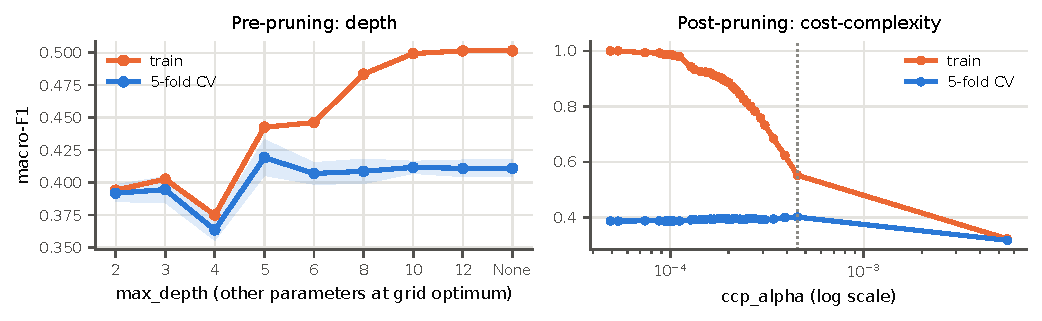
\includegraphics[width=0.93\textwidth]{m3_dt_overfitting}
\caption{Decision Tree: train and CV macro-F1 vs depth (left) and cost-complexity $\alpha$ (right).}\label{fig:overfit}
\end{figure*}

\paragraph{KNN} It works on log, standardized, one-hot data. With the plain vote, macro-F1 falls from 0.38 to 0.24 as $k$ grows while accuracy rises to the majority level (\cref{fig:knn}): large neighbourhoods always contain more \emph{medium} sellers. The prior-corrected rule $\arg\max_c P(c\mid x)/P(c)$ reverses the trend, with a plateau for $k=101$--$201$. Metric and weighting are secondary. The training F1 of 1 under distance weights is trivial (each point is its own nearest neighbour) and is not a sign of overfitting.

\begin{figure*}[t]
\centering
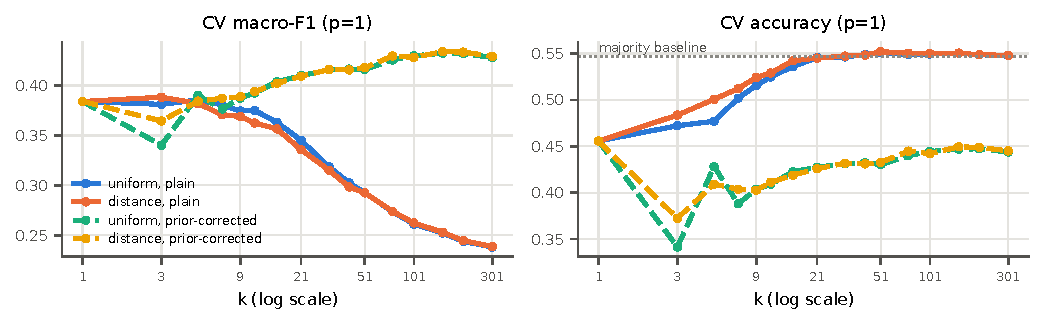
\includegraphics[width=0.93\textwidth]{m3_knn_k}
\caption{KNN: CV macro-F1 (left) and accuracy (right) vs $k$, by weighting and decision rule.}\label{fig:knn}
\end{figure*}

\paragraph{Na\"ive Bayes} GaussianNB uses the 19 numerical attributes, log-transformed and standardized. Scaling matters although the model is scale-invariant in theory: \code{var\_smoothing} adds a fraction of the largest variance to all variances, and unscaled mileage flattened all other attributes (0.31). CategoricalNB uses all 24 attributes, with quantile bins; three coarse bins are best and $\alpha$ is irrelevant (hundreds of sellers per bin). Both assumptions are violated: within each class $\rho_s$(mileage, share of new) is $-0.81$ to $-0.87$ and $\rho_s$(hp, tank) is about 0.8, and 11 of 19 attributes keep $|\mathrm{skew}|>1$ in some class. Correlated evidence is counted several times, which hurts probabilities more than rankings; binning removes the Gaussian assumption, hence CategoricalNB's edge.

\subsection{Baseline results on the test set}\label{sec:test}
\begin{table*}[t]
\centering
\caption{Test set, baseline-grid models: overall metrics and precision/recall/F1 per class (best of each grid by CV macro-F1).}\label{tab:test}
\tabtight{m3_test}
\end{table*}

\begin{figure*}[t]
\centering
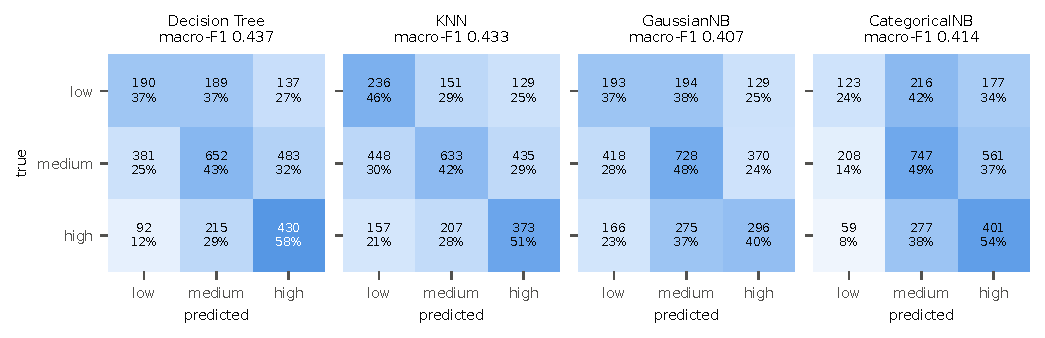
\includegraphics[width=0.95\textwidth]{m3_confusion}
\caption{Confusion matrices on the test set (counts and row percentages).}\label{fig:conf}
\end{figure*}

\begin{figure*}[t]
\centering
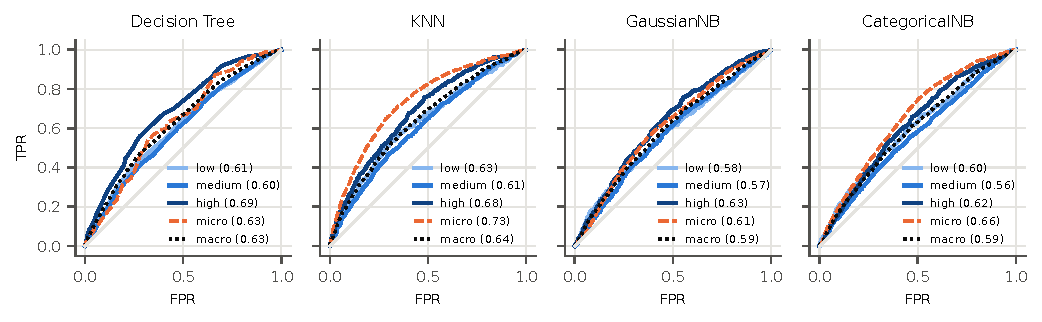
\includegraphics[width=0.95\textwidth]{m3_roc}
\caption{One-vs-rest ROC curves with per-class, micro and macro AUC (test set).}\label{fig:roc}
\end{figure*}

All models (\cref{tab:test}) clearly beat the majority class in macro-F1 (0.41--0.44 vs 0.24) and, as expected when all classes weigh the same, stay below its accuracy. CV and test scores differ by at most 0.02. The Decision Tree and KNN lead; the tree has the best \emph{high} recall (0.58), KNN the best \emph{low} recall (0.46) and the best AUC (macro 0.64, micro 0.73), since a 151-neighbour frequency is a smooth score while the tree only outputs 31 distinct values (stepped curves in \cref{fig:roc}). In \cref{fig:conf} \emph{medium} leaks to both sides: the tree sends 25\% of it to \emph{low} and 32\% to \emph{high}. \emph{High} is the easiest class for every model (AUC 0.62--0.69); CategoricalNB finds only 24\% of \emph{low}. An AUC of 0.6 means that the attributes rank sellers only slightly better than chance, which motivates the experiments below.

\subsection{Sensitivity of the baselines}\label{sec:ablation}
Before improving the models we asked what they depend on. Each row of \cref{tab:abl} changes one element of a baseline and repeats the same 5 folds (everything refitted inside the folds, the test set untouched).

\begin{table}[t]
\centering
\caption{Ablations: change of CV macro-F1 vs the baseline on identical folds. Bold: same sign in all five folds. Trees are invariant to scale.}\label{tab:abl}
\tab{m5_ablation}
\end{table}

\begin{itemize}
\item \textbf{Scale} is decisive for distances: unscaled KNN loses 0.063 and unscaled GaussianNB 0.097, because mileage and price dominate. The log matters less (0.003 and 0.014); standardization beats min--max and robust scaling, which are distorted by extremes or by zero-inflated attributes.
\item \textbf{Outliers}: winsorizing changes nothing, and removing DBSCAN noise from the training folds \emph{hurts} all models ($-0.010$ to $-0.018$). The extreme sellers carry information, which supports keeping them (\cref{sec:quality}).
\item \textbf{Attributes}: seller size and the block price--turnover--wear are needed; vehicle specifications, 8 of the 19 numerical attributes, contribute nothing to the tree and KNN. Size alone gives only 0.36.
\item \textbf{Segments as features} help the tree slightly ($+0.006$, all folds) and hurt KNN and GaussianNB, where they duplicate existing distances.
\end{itemize}

\subsection{Extended models: partial prior correction and engineered attributes}\label{sec:tau}
\paragraph{Idea} The baselines treat imbalance as all or nothing: no correction ignores the minority classes, full balancing sends half of \emph{medium} elsewhere. We interpolate with an exponent $\tau$:
\begin{equation}
\hat y=\arg\max_c \frac{P(c\mid x)}{P(c)^{\tau}},\qquad \tau\in[0,1].
\end{equation}
$\tau=0$ is the plain rule and $\tau=1$ the prior-corrected rule of KNN. For the tree the same exponent defines the class weights $w_c\propto P(c)^{-\tau}$ ($\tau=1$ is \code{balanced}), for Na\"ive Bayes it rescales the prior. We added 12 attributes computed from a seller's own row, so they cannot leak: listings per active day, share of active days, listing rate, savings/price, number of new, used, theft, salvage and ex-taxi vehicles, price per hp, miles per year, days on market over span.

\paragraph{Search} $\tau\in\{0,.25,.5,.6,.7,.8,.9,1\}$ and engineered attributes on/off, crossed with: tree depth $\{4,5,6,8,10\}$ and leaf $\{20,50,100\}$; KNN $k\in\{51,101,151,201\}$ (distance weights, $p=1$); GaussianNB smoothing $\{10^{-3},10^{-2},10^{-1}\}$; CategoricalNB bins $\{3,4,6\}$: 400 configurations. Intermediate $\tau$ wins clearly for the tree ($\tau=0.7$, 0.445 vs 0.419 at 1) and KNN ($\tau=0.8$, 0.456 vs 0.438), while Na\"ive Bayes is flat (\cref{fig:tau}, left): its over-confident posteriors are barely moved by a prior factor. Chosen: tree with depth 4, leaf 20, $\tau=0.7$; KNN with $k=151$, $\tau=0.8$; GaussianNB with smoothing $10^{-3}$, $\tau=0$; CategoricalNB with 4 bins, $\tau=0$; all with engineered attributes.

\begin{figure*}[t]
\centering
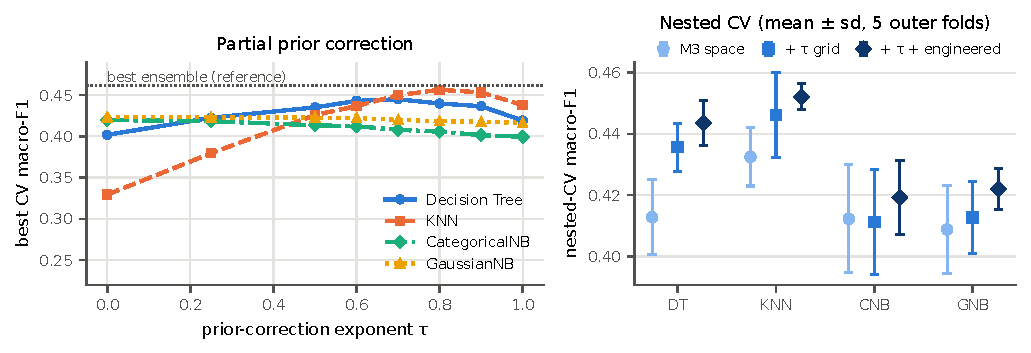
\includegraphics[width=0.93\textwidth]{m5_tau}
\caption{Left: best CV macro-F1 for each value of $\tau$. Right: nested CV of the three search spaces.}\label{fig:tau}
\end{figure*}

\paragraph{Nested CV} Larger grids look better by chance, so we compared whole search spaces with \emph{nested} CV (inner 5-fold search, outer 5-fold score; \cref{tab:nested}). The $\tau$ grid improves tree and KNN in all five folds and the engineered attributes add a little more: $+0.031$ for the tree and $+0.020$ for KNN in total. Na\"ive Bayes gains only from the attributes (about $+0.01$).

\begin{table}[t]
\centering
\caption{Nested CV macro-F1 (mean$\pm$sd; folds better than the baseline space in brackets).}\label{tab:nested}
\tabtight{m5_nested}
\end{table}

\paragraph{Test set} The test set had been used once for the baselines (\cref{tab:test}); here it is used once more, for the single configuration per model fixed by CV. \Cref{tab:ext,fig:ci} add bootstrap confidence intervals (2\,000 resamples of the test sellers). Two ensembles outside the lecture programme (a 300-tree random forest and gradient boosting, only $\tau$ tuned) are a yardstick, not candidates. Paired bootstrap on the same resamples:
\begin{itemize}
\item the baseline tree, KNN and the rules of \cref{sec:exploit} are tied (all intervals of the differences contain 0 and lie within $\pm0.025$), while the tree beats GaussianNB (CI $[0.006,0.052]$);
\item extended KNN beats baseline KNN by 0.031, CI $[0.013,0.047]$; the extended tree gains 0.007, not significant ($[-0.011,0.025]$), although its CV gain was larger: the baseline tree had been lucky on the test set (CV 0.419, test 0.437);
\item extended KNN is ahead of the extended tree by 0.020, $[0.000,0.041]$, and level with gradient boosting ($[-0.015,0.018]$) and the random forest ($[-0.004,0.027]$).
\end{itemize}
A partial correction also restores accuracy (0.45 to 0.52 for KNN), because fewer \emph{medium} sellers are sacrificed. The price is a lower \emph{low} recall (0.46 to 0.27 for KNN, 0.37 to 0.19 for the tree). For KNN the F1 of \emph{medium} (0.505 to 0.608) and \emph{high} (0.446 to 0.486) rises and that of \emph{low} falls (0.348 to 0.298), so the baseline rule remains preferable when the goal is to find low-rated sellers.

\begin{table*}[t]
\centering
\caption{Extended models on the test set, with bootstrap 95\% CI of macro-F1, quadratic-weighted kappa (QWK) and mean absolute error on the ranks (MAE). \emph{Extended}: $\tau$ and attributes chosen by CV.}\label{tab:ext}
\tabtight{m5_test}
\end{table*}

\begin{figure}[t]
\centering
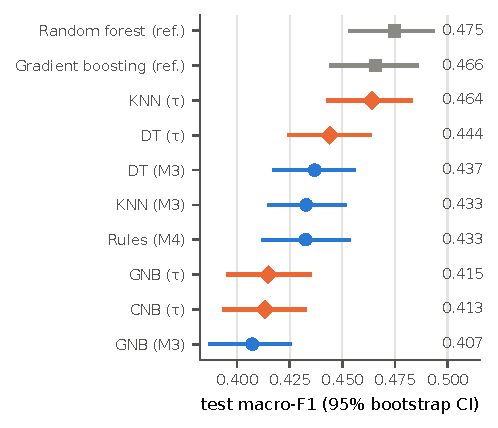
\includegraphics[width=0.97\linewidth]{m5_test_ci}
\caption{Test macro-F1 with 95\% CI. Circles: baselines; diamonds: extended; squares: reference ensembles.}\label{fig:ci}
\end{figure}

\subsection{What the trees say}\label{sec:tree}
The baseline tree splits first on size (\attr{n\_listings} $\leq103.5$), which accounts for 62\% of its impurity decrease, followed by price (13\%), share of new (7\%) and mileage (6\%). Its purest large leaf describes \emph{high} sellers: at most 17 listings, mileage below 79k, independent, not mainly sedans (279 sellers, 65\% \emph{high}; base rate 27\%).
The extended tree (16 leaves, \cref{fig:tree}) starts from an engineered attribute, the \emph{number of used cars} (63\% of the impurity decrease): size matters through the used stock more than through all listings. Read left to right, \emph{high} is predicted for sellers with few used cars, most purely with at most 17 and a savings/price ratio up to 10\% (1\,706 sellers, 49\% \emph{high}); \emph{medium} for expensive inventories (price $>36.2$k: 72--81\% \emph{medium}); \emph{low} for large, cheaper sellers ($>154$ listings and $>45$ used cars, 30\% \emph{low}), refined by price $\leq25.2$k in the next level (915 sellers, 37\% \emph{low} against 19\% overall, 35\% on the test set). Large leaves keep their precision on the test set (biggest leaf per class, train to test: \emph{high} 0.39 to 0.37, \emph{medium} 0.63 to 0.60, \emph{low} 0.37 to 0.35), small ones do not (47 sellers: 0.70 to 0.38). No leaf with more than 30 sellers is mostly \emph{low}: the data contain no clear profile of a low-rated seller.

\begin{figure*}[t]
\centering
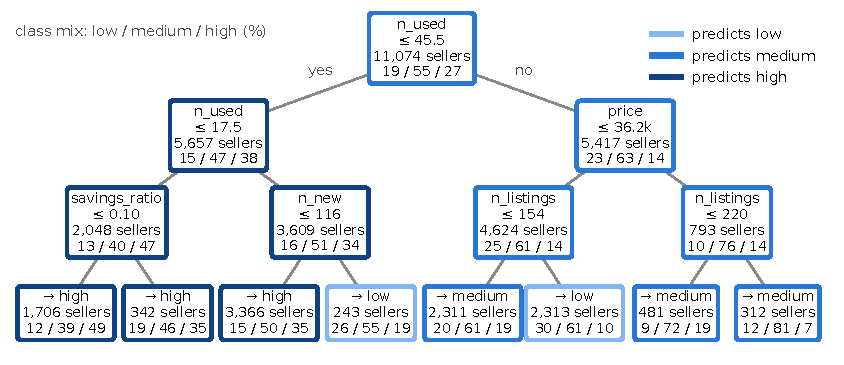
\includegraphics[width=0.97\textwidth]{m5_tree}
\caption{Extended Decision Tree, top three levels (left branch: condition true). Class mixes are unweighted shares of the training sellers; border: class predicted under the $\tau$-weighted rule.}\label{fig:tree}
\end{figure*}

\subsection{Error analysis: ordinality, ceiling, agreement}\label{sec:errors}
\paragraph{Ordinal errors} The rating is ordinal, so confusing \emph{low} and \emph{high} is worse than confusing neighbours. The baseline tree makes this error in 15\% of its mistakes, but the share must be read against chance: with the same marginals and independent predictions it would be 21\%. The ratio is 0.70--0.94 over all models, so they do capture the order, though weakly (QWK 0.14--0.26). The extended tree is best (12\% vs 17\% expected). We also tried an \textbf{ordinal decomposition} (Frank and Hall: two trees for $y>$ \emph{low} and $y>$ \emph{medium}, same grid): out-of-fold QWK 0.235 vs 0.233 and macro-F1 0.448 vs 0.445. Modelling the order explicitly adds nothing.

\paragraph{Ceiling} Extended KNN is statistically level with the ensembles, so a more flexible model does not extract much more from these attributes. The learning curves (\cref{fig:cross}, centre) are flattening but not flat: from 3\,500 to 8\,900 training sellers KNN gains only 0.013. More sellers would help slowly; better attributes are what is missing. A rating reflects service quality, and no column describes it.

\paragraph{By segment} The macro-F1 of the baseline tree is similar in the four K-Means segments (0.39--0.45): best in C1, worst in C3, where classes overlap most.

\paragraph{Agreement} Extended tree, extended KNN and the rule classifier, three different learners, agree on 52\% of the test sellers. Precision there is 0.58 overall, 0.68 on \emph{medium} (base rate 0.55), 0.48 on \emph{high} (0.27) and 0.39 on \emph{low} (0.19); where they disagree KNN is right in 45\% of the cases. Agreement is a usable confidence signal, but even three concordant models are often wrong on \emph{low}.

\begin{figure*}[t]
\centering
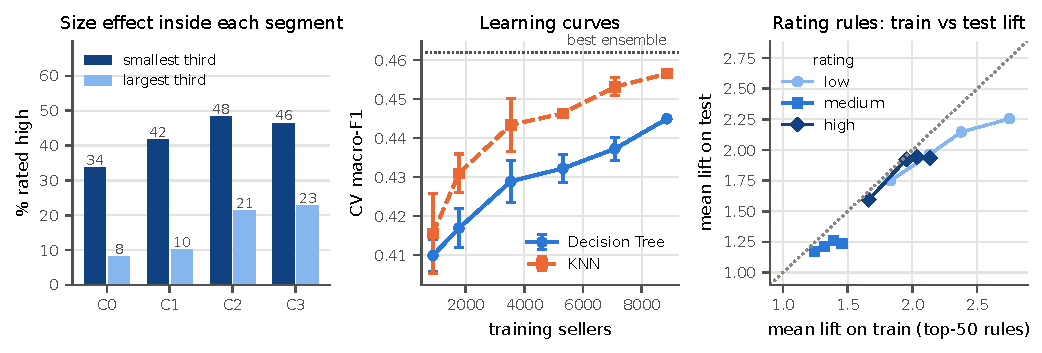
\includegraphics[width=0.95\textwidth]{m5_cross_module}
\caption{Left: share of \emph{high} among the smallest and largest third of the sellers of each K-Means segment. Centre: learning curves of the extended models. Right: lift of the 50 best rating rules per support band, train vs test (dotted: identity; see \cref{sec:exploit}).}\label{fig:cross}
\end{figure*}

\subsection{Seller size confounds dealer type}\label{sec:simpson}
\begin{table}[t]
\centering
\caption{Rating vs size. Top: Spearman's $\rho_s$ between \attr{n\_listings} and rating, and shares among the smallest (S) and largest (L) third of each group. Bottom: dealer type within size tertiles.}\label{tab:size}
\tab{m5_size}\\[5pt]
\tab{m5_dealer}
\end{table}

\Cref{sec:m1,sec:m2} found that independents are rated \emph{high} more often than franchises (33\% vs 21\%). Is this dealer type or size? The \textbf{size effect is universal}: within every segment and both dealer types small sellers are \emph{high} 2 to 4 times as often as large ones (\cref{tab:size}, top; \cref{fig:cross}, left). The \textbf{dealer effect reverses}: in no size tertile do independents have more \emph{high} sellers, and among mid and large ones franchises have clearly more (\cref{tab:size}, bottom). The crude odds ratio of \emph{high} for franchises is 0.53 (95\% CI 0.49--0.57); adjusted for size deciles (Mantel--Haenszel) it becomes \textbf{1.73} (1.54--1.95). This is a Simpson's paradox: independents look better because they are small (median 26 vs 154 listings). It corrects the naive reading of \cref{fig:target} and explains why the tree needs size first.

\subsection{Regression}\label{sec:reg}
\paragraph{Task} The target is \attr{price} (seller median), on the \code{log1p} scale: it is the central economic attribute, is strongly related to the others, and its log is almost symmetric (skew $3.4\to-0.4$), so additive effects become relative ones. No predictor derives from price. Split and folds are those of the classification; tuning minimizes CV MSE.

\paragraph{Single regression} On the training set \attr{mileage} has the strongest correlation with price ($\rho_s=-0.82$) and is the textbook driver of used-car prices. OLS gives $\widehat{\log(1+\mathrm{price})}=10.40-0.1035\,\mathrm{mileage}/10^4$: about $-9.8\%$ per 10\,000 miles. It explains 75\% of the variance on train and test alike, but only 48\% in dollars. The residuals (\cref{fig:slr}) show where the line fails: new-car sellers pile up at zero mileage with any price, nearly new stock (100--20k miles) is under-predicted ($+0.09$), and the spread grows with mileage (std 0.25 to 0.42).

\begin{figure*}[t]
\centering
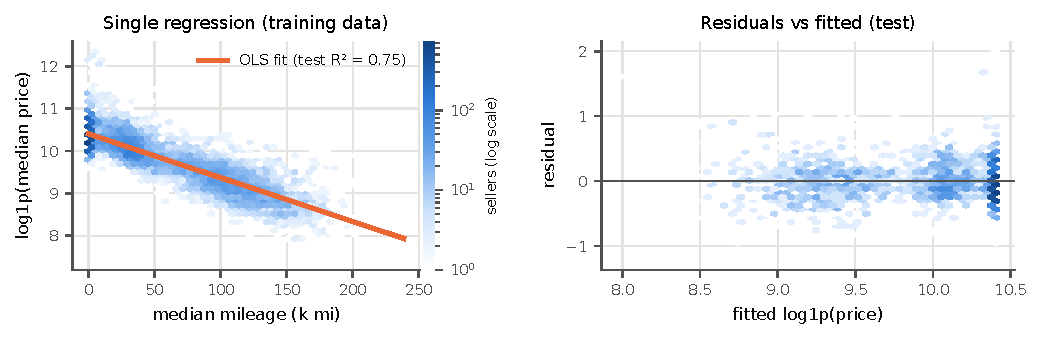
\includegraphics[width=0.93\textwidth]{m3_slr}
\caption{Single regression of log price on mileage: fit on the training set (left), test residuals (right).}\label{fig:slr}
\end{figure*}

\paragraph{Multiple regression} Four predictors cover different aspects: \attr{mileage} (wear), \attr{horsepower}, \attr{width} (vehicle class) and \attr{pct\_is\_new} (composition); all VIFs are below 2.5. We compare OLS with two non-linear models: a Decision Tree regressor (depth $\{2,3,4,5,6,8,10,12,15,\text{none}\}$ $\times$ leaf $\{1,5,10,20,50,100\}$, 60 configurations; best depth 12, leaf 20, CV MSE 0.0374; e.g.\ 0.048 at depth 5) and KNN on standardized inputs ($k\in\{1,3,5,7,10,15,20,30,50,75,100\}$ $\times$ $p\in\{1,2\}$ $\times$ weights, 44 configurations; best $k=30$, $p=1$, distance weights, CV MSE 0.0337). \Cref{tab:reg,fig:regpred}: three more predictors halve the linear error ($R^2$ 0.747 to 0.876). In the standardized OLS, mileage ($-0.48$) and horsepower ($+0.21$) carry nearly all the effect. The non-linear models add 0.03--0.04 of $R^2$ by modelling the zero-mileage regime and interactions; KNN has the lowest test error, the tree a smaller model that can be read. KNN's zero training error is again an effect of distance weights.

\begin{table}[t]
\centering
\caption{Regression on log price (same split and target). $R^2$(\$): after back-transformation to dollars.}\label{tab:reg}
\tabtight{m3_reg}
\end{table}

\begin{figure*}[t]
\centering
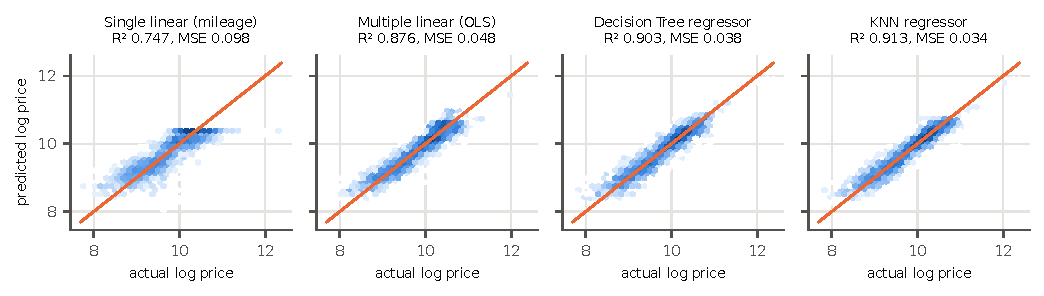
\includegraphics[width=0.95\textwidth]{m3_regression_pred}
\caption{Predicted vs actual log price on the test set.}\label{fig:regpred}
\end{figure*}

\paragraph{Sensitivity} \Cref{tab:regabl} crosses three predictor sets with the target scale (training-set CV). On the raw scale OLS predicts \emph{negative} prices for 107--206 sellers and, judged on the log scale, is worse than the mean: the log target is essential for linear models and irrelevant for tree and KNN. With all 18 numerical predictors OLS and the tree improve (CV $R^2$ 0.880 to 0.896 and 0.903 to 0.910), KNN does not (0.913 to 0.914). On the test set the 18-predictor models give 0.896 (OLS), 0.910 (tree) and 0.908 (KNN), so none beats KNN on four attributes (0.913). Four interpretable predictors are enough.

\begin{table}[t]
\centering
\caption{Regression ablation, training-set CV: 1 (mileage), 4 or 18 predictors. APE: median absolute percentage error; neg.: negative predicted prices.}\label{tab:regabl}
\tabtight{m5_reg}
\end{table}

\subsection{Which algorithms are best?}\label{sec:best}
\Cref{tab:best} compares the classifiers from several perspectives.

\begin{table}[t]
\centering
\caption{Classifiers by perspective (extended models, test set).}\label{tab:best}
{\tabfont\setlength{\tabcolsep}{2.5pt}
\begin{tabular}{@{}p{0.20\linewidth}p{0.24\linewidth}p{0.24\linewidth}p{0.22\linewidth}@{}}
\toprule
 & Decision Tree & KNN & Na\"ive Bayes\\
\midrule
\Fm\ / AUC & 0.444 / 0.634 & \textbf{0.464 / 0.658} & 0.415 / 0.609\\
CV--test gap & $<0.001$ & 0.008 & 0.008\\
Readability & \textbf{16 rules} & none & likelihoods\\
Skew, outliers & \textbf{invariant} & log, scaling & log or bins\\
Assumptions & none & meaningful distance & independence: violated\\
Cost & \textbf{negligible} & 11k distances per query & negligible\\
\bottomrule
\end{tabular}}
\end{table}

\paragraph{Classification} \textbf{KNN} ($k=151$, $\tau=0.8$) is the best predictor: it leads macro-F1, accuracy and AUC, in CV as on the test set, and is statistically level with the ensembles. The \textbf{Decision Tree} is close, explains itself and costs nothing: it is the model to show to a user, and it has the best ordinal agreement among the lecture models (QWK 0.26). On the baseline grids alone the two are tied and the tree would be preferred. Na\"ive Bayes pays for correlated attributes.

\paragraph{Regression} KNN has the lowest error ($R^2$ 0.913), the Decision Tree regressor (0.903) offers the best trade-off with a small train--test gap (MSE 0.028 vs 0.038), and OLS (0.876) is the most interpretable. Price is strongly determined by the inventory, the rating only weakly.


\section{Pattern mining}\label{sec:m4}

\subsection{Transactional encoding}\label{sec:enc}
Each seller becomes a transaction with at most one item per attribute, written \emph{attribute=value}:
\begin{itemize}
\item \textbf{Equal-frequency tertiles} (\emph{low}/\emph{mid}/\emph{high}) for seven skewed attributes: size, price, mileage, days on market (\emph{dom}), horsepower (\emph{hp}), listing span, share of ex-taxis (\emph{cab}). Equal-width bins would put almost all sellers in one bin.
\item \textbf{Domain bins} for savings: \emph{none} (37\% exact zeros), and \emph{low}/\emph{high} split at the median of the positive values.
\item \textbf{Presence items} \emph{salvage=yes} and \emph{theft=yes} for the zero-inflated shares.
\item The grouped categoricals (body, colour, transmission, dealer, inventory) and \emph{rating}.
\end{itemize}
Missing values simply produce no item. Items with support above 0.9 (\emph{trans=a}, 94\%) are removed: they would double every pattern with lift $\approx1$. The result is 50 items and 13.3 items per seller, a dense dataset. Bin edges are learned on the data being mined: all sellers for description (\cref{sec:freq,sec:rules}), training folds only for prediction (\cref{sec:exploit}). We used Apriori; the available FP-Growth implementation returns the same itemsets but was about 70 times slower with so few and dense items.

\subsection{Frequent itemsets}\label{sec:freq}
\begin{figure*}[t]
\centering
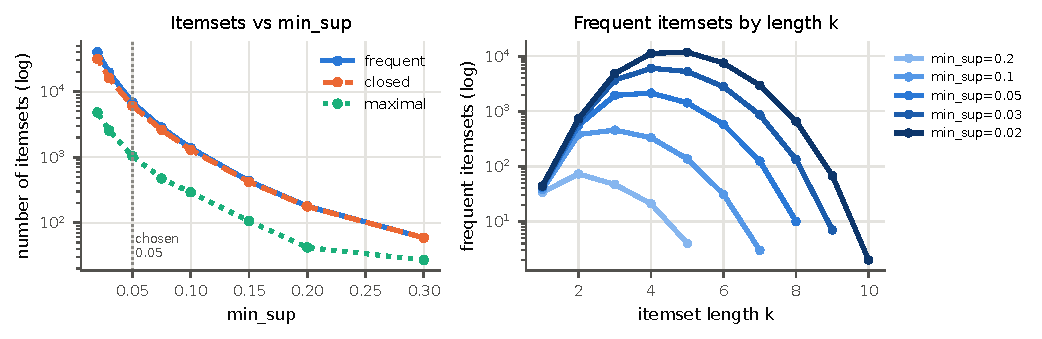
\includegraphics[width=0.93\textwidth]{m4_itemsets_sweep}
\caption{Number of frequent, closed and maximal itemsets vs \code{min\_sup} (left) and frequent itemsets by length $k$ (right).}\label{fig:isets}
\end{figure*}

\begin{table}[t]
\centering
\caption{Itemsets by \code{min\_sup} (all tested values).}\label{tab:isets}
\tab{m4_sweep}
\end{table}

\paragraph{Quantitative analysis} The number of itemsets grows about exponentially as \code{min\_sup} decreases (\cref{fig:isets,tab:isets}) and the mode of the length distribution moves from $k=2$ at 0.2 to $k=5$ at 0.02: tertile items all have support near 1/3, so long conjunctions of typical values stay frequent. Closed itemsets are 79--100\% of the frequent ones, i.e.\ few items imply each other exactly; maximal ones are 5--8 times fewer at \code{min\_sup}$\,\leq0.1$. We chose \textbf{\code{min\_sup}$\,=0.05$} (6\,835 itemsets, 1\,042 maximal): every pattern describes at least 693 sellers, \emph{rating=low} (18.6\%) can still combine with other items, and lower values multiply the output by 3--6 with mostly redundant combinations.

\paragraph{Qualitative analysis} \Cref{tab:iset} shows the most frequent closed itemsets with at least four items, and the most frequent ones containing each rating. Two seller types emerge without any distance: the \emph{franchise new-car dealer} (31\%) and the \emph{independent budget used-car dealer} (30\%), the K-Means segments C0 and C3. The longest maximal itemset (8 items, 7.7\%) refines the former with SUV, high price, large size and \emph{rating=medium}. Among the ratings, \emph{high} occurs mostly with independent used-car sellers, \emph{low} with mixed-inventory franchises; their lift decides whether this exceeds chance.

\begin{table}[t]
\centering
\caption{Most frequent closed itemsets with $k\geq4$ (top), and with a rating item and $k\geq3$ (bottom).}\label{tab:iset}
\tab{m4_itemsets}
\end{table}

\subsection{Association rules}\label{sec:rules}
\paragraph{Quantitative analysis} From the 0.05-frequent itemsets we generated 87\,266 rules with confidence at least 0.3 and counted them for eight \code{min\_conf} values and every length (\cref{fig:rules}). Counts peak at $k=5$, since an itemset of size $k$ yields $2^k-2$ rules, and fall slowly: only 12.5 times from \code{min\_conf} 0.3 to 0.95, because the encoding contains near-deterministic relations (6\,971 rules have confidence $\geq0.95$). We chose \textbf{\code{min\_conf}$\,=0.6$}: 34\,233 rules remain and 99.8\% of them have lift above 1 (100\% from 0.7), so confidences that only reflect a frequent consequent are excluded. The confidence histogram is spread over $[0.6,1]$ (median 0.78) with a peak at 1. Lift concentrates between 2 and 3 (median 2.2): a tertile consequent caps it at 3, and the tail up to 6.4 comes from multi-item consequents. High confidence occurs at every support, high lift only at low support.

\begin{figure*}[t]
\centering
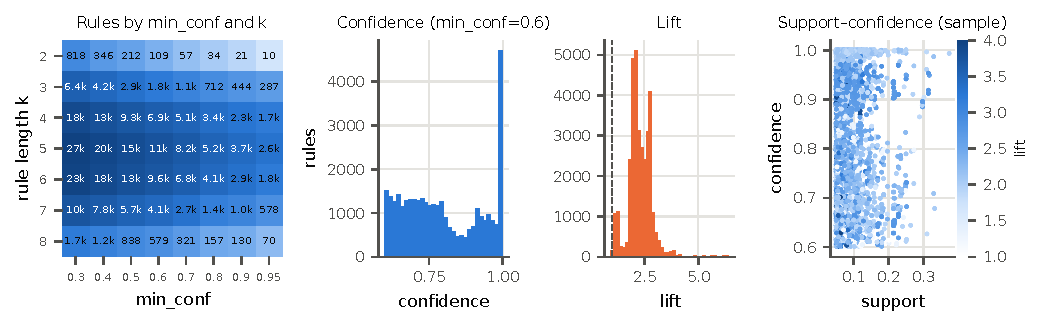
\includegraphics[width=0.97\textwidth]{m4_rules_quant}
\caption{Association rules: counts by \code{min\_conf} and length $k$; histograms of confidence and lift for \code{min\_conf}$\,=0.6$; support--confidence--lift scatter (6\,000 sampled rules).}\label{fig:rules}
\end{figure*}

\paragraph{Qualitative analysis} Ranking by lift alone returns dozens of variants of the same rule. We keep single-item consequents, drop a rule when a subset of its antecedent reaches 99\% of its lift, and show the best rule per consequent (\cref{tab:rules}). They describe inventories and agree with the regressions of \cref{sec:reg}: price, power and mileage determine each other; CVT gearboxes go with small engines; discounting franchises sell mid-mileage cars; franchises with theft-title vehicles are the large ones (more cars, more chance to have one).

\begin{table}[t]
\centering
\caption{Best rule for each consequent, by lift (\code{min\_sup}$\,=0.05$, \code{min\_conf}$\,=0.6$).}\label{tab:rules}
\tabtight{m4_rules}
\end{table}

\paragraph{Rating rules} No rule with consequent \emph{rating=low} or \emph{high} reaches confidence 0.6, so we mined them apart (\code{min\_sup}$\,=0.01$, at most three antecedent items; \cref{tab:rating}). \emph{High} is predicted by small sellers with mid-priced or mid-mileage stock (confidence 0.54 against a base rate of 0.27), \emph{low} by large sellers with mid-priced sedans, CVT or low-power cars (0.40 vs 0.19), \emph{medium} by large expensive sellers (0.77 vs 0.55). Supports are 1--2\% and no rule for \emph{low} or \emph{high} exceeds 0.55 confidence.

\begin{table}[t]
\centering
\caption{Top rating rules by lift (\code{min\_sup}$\,=0.01$).}\label{tab:rating}
\tabtight{m4_rating}
\end{table}

\paragraph{Sensitivity to binning} \Cref{tab:bin} repeats mining and a smaller rule classifier ($s=0.01$, $L=3$, training folds only) under six binnings. Equal-width bins fail, as argued in \cref{sec:enc}: one bin holds up to 100\% of the sellers, lift shrinks and the classifier falls to 0.26--0.29. Two bins triple the itemsets with less specific patterns. Four equal-frequency bins predict better than three (0.420 vs 0.390) with half the itemsets: a possible improvement that we did not tune further, because it was found after the test set had been read. We keep tertiles, whose \emph{low}/\emph{mid}/\emph{high} labels are readable in all descriptive rules.

\begin{table*}[t]
\centering
\caption{Binning sensitivity (without rating items): items, itemsets at \code{min\_sup}$\,=0.05$, rules at \code{min\_conf}$\,=0.6$ and their lift, largest support of a numerical bin, and CV macro-F1 of the rule classifier ($s=0.01$, $L=3$).}\label{tab:bin}
\tabwide{m5_binning}
\end{table*}

\subsection{Exploiting the rules}\label{sec:exploit}
\paragraph{Predicting the rating} The classifier uses the split of \cref{sec:m3}; edges, items and rules come from training data only and hyperparameters from the same 5 folds, with re-mining inside each. Every frequent antecedent $A$ (no rating items) carries the class distribution $P(c\mid A)$ of the sellers it matches, i.e.\ the confidences of its three rules. The delicate choice is how to combine matching rules. We compared eight aggregations over $s\in\{0.005,0.01,0.02\}$ and antecedent length $L\leq4$ (96 configurations, \cref{tab:agg}):
\begin{itemize}
\item \emph{class-best-conf/lift} (CBA style): best matching rule with lift $>1$ per class, then argmax;
\item \emph{best-antecedent}: the matching antecedent with the highest lift, which predicts its most confident class;
\item \emph{top10}, \emph{mean}: average $P(c\mid A)$ over the ten most discriminative, or all, matching antecedents;
\item \emph{+ prior}: the same, divided by $P(c)$.
\end{itemize}

\begin{table*}[t]
\centering
\caption{Rule-based classifier, CV macro-F1 for all 96 configurations (leading zero omitted).}\label{tab:agg}
\tabwide{m4_agg}
\end{table*}

\begin{figure*}[t]
\centering
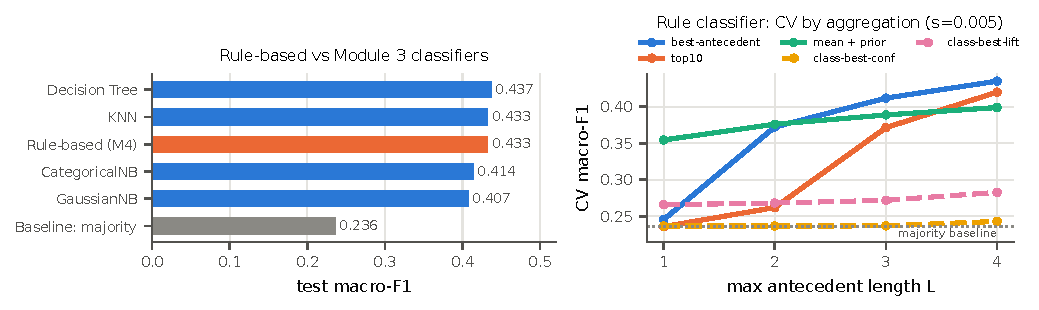
\includegraphics[width=0.93\textwidth]{m4_rule_classifier}
\caption{Test macro-F1 of the rule-based and the \cref{sec:m3} baseline-grid classifiers (left); effect of aggregation and antecedent length in CV (right).}\label{fig:rulecls}
\end{figure*}

The aggregation matters more than any other parameter. Per-class maxima fail (0.24--0.28) because they are not comparable: confidence is bounded by class frequency, so \emph{medium} always wins, and lift by $1/P(c)$, which favours \emph{low}. \emph{best-antecedent} avoids this since its three confidences come from the same sellers: $s=0.005$, $L=4$ gives CV macro-F1 0.435, growing with $L$ (\cref{fig:rulecls}, right). On the test set it reaches macro-F1 0.433 and accuracy 0.492 with 100\% coverage: equal to the Decision Tree (0.437) and KNN (0.433) of the baseline grid, with more weight on \emph{medium} (recall 0.58) and less on \emph{low} (0.25). The model holds 46k rules and is not readable as a whole, but every single prediction is explained by one rule.

\paragraph{Generalization of the rules} Ranking thousands of rules by lift selects lucky ones. We took the 50 rating rules with the highest training lift in each support band and re-measured them on the test set (\cref{tab:gen}; \cref{fig:cross}, right). In every band they remain positively associated on average, but the excess over 1 shrinks, most where support is lowest: by 28\% for \emph{low} and 49\% for \emph{medium} at 0.5--1\%, against 3--10\% for \emph{high} above 1\%. Extreme lifts at low support are partly selection, so a rule should be judged on support too.

\begin{table}[t]
\centering
\caption{Mean lift of the 50 best rating rules per support band, training $\to$ test.}\label{tab:gen}
\tabtight{m5_gen}
\end{table}

\paragraph{Imputing missing values} We masked an attribute for all 2\,769 test sellers and predicted it with the most confident matching rule mined on the training set (\code{min\_sup}$\,=0.01$, at most three antecedent items, rating excluded). \Cref{tab:imp}: the \textbf{price tertile} is recovered in 75.2\% of the cases against 35.1\% for the mode; the \textbf{body type} is not (65.0\% vs 64.2\%), because its determinants, the dimensions, are not encoded as items. Rules impute well exactly when the transactions contain the drivers of the attribute.

\begin{table}[t]
\centering
\caption{Rule-based imputation of masked test values.}\label{tab:imp}
\tabtight{m4_imp}
\end{table}

\subsection{Describing the segments with rules}\label{sec:segrules}
Adding the K-Means segment as an item and mining $A\to$ \emph{segment} (\code{min\_sup}$\,=0.02$) gives short definitions of the clusters (\cref{tab:segrules}). C0, C1 and C3 are almost deterministic (confidence $\geq0.97$). C2 needs slow turnover \emph{and} a long span and stays at 0.84, with lift 9: the same fragility found with DBSCAN. With these rules a seller can be assigned to a segment without computing distances.

\begin{table}[t]
\centering
\caption{Two most confident non-redundant rules per K-Means segment.}\label{tab:segrules}
\tabtight{m4_segments}
\end{table}

\section{Conclusions and limitations}\label{sec:concl}
\paragraph{One story from four modules} Every analysis finds the same axis. The correlation blocks (\cref{sec:corr}), the two DBSCAN cores and the first K-Means and Ward split (\cref{sec:m2}), the most frequent itemsets (\cref{sec:freq}) and the price regressions (\cref{sec:reg}) all oppose large franchises with new cars to small independents with old ones. The modules also check each other: segments are confirmed by rules with confidence up to 1.00 (\cref{sec:segrules}); the fragile segment C2 is the one that DBSCAN calls noise, that disappears in the outlier test and that has the weakest rules; the rating rules, the trees and the effect sizes all place seller size first.

\paragraph{The rating} Three families of methods (distances, trees, rules) and two ensembles reach at most 0.475 macro-F1 (Na\"ive Bayes about 0.41), so the limit lies mainly in the attributes: they describe what is sold and not how customers are served. Within this limit, the decision rule mattered more than the algorithm: tuning $\tau$ gave the tree and KNN more than any other choice. The strongest lesson on interpretation is the dealer-type paradox (\cref{sec:simpson}): a significant and repeatedly observed association changed sign after conditioning on size.

\paragraph{The best algorithms} \emph{Clustering}: K-Means, $k=4$ (coverage, reproducibility, readable segments). \emph{Classification}: KNN with $\tau=0.8$ for prediction, with a 16-leaf tree as its readable companion. \emph{Regression}: KNN for error, Decision Tree as compromise, OLS for explanation. \emph{Patterns}: Apriori with equal-frequency bins; the aggregation of the rules is the critical choice of the classifier.

\paragraph{Limitations}
\begin{itemize}
\item Seller-level medians hide inventory variance, and units are inferred.
\item \emph{Low} is never identified well (recall $\leq0.46$): no attribute gives it a profile of its own.
\item All associations are observational; we cannot say why small sellers are rated higher (service, number of reviews, selection). The number of reviews behind each rating is unknown.
\item The test set was read more than once (baseline models, rules, extended models). Configurations were fixed by CV each time, and nested CV gives the same ranking, but the intervals of \cref{tab:ext} do not include model-selection uncertainty.
\item C2 depends on the tail of two attributes; another scaling could absorb it.
\end{itemize}
Data on reviews, prices relative to the market, or response times would be the natural next step.

\end{document}
